\documentclass[12pt]{article}
\usepackage[margin=1in]{geometry}
\usepackage{amsfonts,amsmath}
\usepackage{parskip}
\usepackage[]{graphicx}
\usepackage{mathrsfs}
\usepackage{listings} 
\usepackage{color}
\usepackage{ulem}
\usepackage{hyperref}
\usepackage{booktabs}
\usepackage{tikz}
\begin{document}
%\pagenumbering{gobble}
\setlength{\parindent}{3em}
\setlength{\parskip}{1em}


\newcommand{\ttspc}{\hspace{1mm}}
\newcommand{\tspc}{\hspace{2mm}}
\newcommand{\lspc}{\hspace{10mm}}
\newcommand{\ttc}{, \ttspc}
\newcommand{\nth}{^{\text{th}}}
\newcommand{\mybegit}{\vspace{-2mm} \begin{itemize} \itemsep-.6em }
\newcommand{\mytitle}[1]{\vspace{10mm} \noindent\begin{large} \textbf{{#1}} \end{large}} 
\newcommand{\soutt}[1]{%
    \renewcommand{\ULthickness}{1.0pt}%
       \sout{#1}%
    \renewcommand{\ULthickness}{.4pt}% Resetting to ulem default
}



\begin{center}
\begin{Large} \textbf{CSC-213: PROF. CURTSINGER} \\
\vspace{3mm} \textbf{FINAL PROJECT REPORT} \end{Large} \\
\vspace{5mm} ANNA BLINDERMAN, DAVID KRAEMER, ZACHARY SEGALL
\end{center} 

\mytitle{Project Overview ($<$400 words)}
\mybegit
	\item introduce Game of Life
	\item describe GUI
	\item describe GPU stencil update
	\item describe listener CPU threads
	\item describe evaluation strategies
	\item summarize evaluation results
\end{itemize}

	We implement a variation of Conway's Game of Life -- a cellular automaton simulation created by the mathematician John Conway. Scientific computing and large-scale simulations are incredibly useful across a variety of fields. However, many of these programs are prohibitively slow. Therefore the algorithms and design of these programs is crucial. Although Life was initially created as a tool to explore computability, Turing machines, and Von Neumann machines, the various types of optimization we explore in our project are applicable to a wide variety of graphics-intensive programs. 
	
	The Game of Life is simply a series of iterations of a rendering of a grid of cells. Each cell is either dead or alive, and there exists a simple deterministic algorithm that decides each cell's state at the next iteration. We implement a version of the Game of Life and render the simulation on
        an interactive graphical interface using the SDL framework, providing
        basic user controls such as pausing and unpausing the simulation,
        stepping through one increment of the simulation, activating and
        deactivating cells, and clearing and quitting the application.

	[friend can you please write the paragraph on the ui don't you read through libraries in your spare time or something]
	
	For each iteration, we use Conway's algorithm to determine the state (dead or alive) of every cell in our grid. Because this algorithm takes as input a cell along with the states of each of its eight immediate neighbors, this algorithm naturally lends itself to an ``embarrasingly parallel" stencil computation on the GPU.
	
	We also have two threads running on the CPU -- one for recording and acting on user input from the mouse; the other from the keyboard. 
	
	To evaluate our system, we first varied the number of threads per block in our stencil function calls. Then, we implemented a feature that allowed us to find regions with no live cells in order to skip their calls to the update functions. 
	
	[LOL SUMMARY OF RESULTS WHAT HAPPENED?!?!?] [friend]





\newpage\mytitle{Design and Implementation ($\sim$2 pages)} (Zachary)
\mybegit
	\item summary of overall implementation structure
	\item Component 1: GUI
		\mybegit
			\item responsibilities/how fits into entire structure
			\item rationale for choice 
			\item data structures/algorithms/libraries/other details
		\end{itemize}
	\item Component 2: mouse/keyboard input
		\mybegit
			\item responsibilities/how fits into entire structure
			\item rationale for choice 
			\item data structures/algorithms/libraries/other details
		\end{itemize}
	\item Component 3: GPU stencil update
		\mybegit
			\item responsibilities/how fits into entire structure
			\item rationale for choice 
			\item data structures/algorithms/libraries/other details
		\end{itemize}
	\item Butler Lampson's Hints for Computer System Design (integrate?)
		\mybegit
			\item don't reinvent the wheel (+ how it did/didn't help)
			\item be prepared to throw an entire thing out  (+ how it did/didn't help)
		\end{itemize}
	\item figures if appropriate
\end{itemize}

\newpage
	The rules to Conway's Game of Life are simple. There exists a grid of cells, where every cell is either dead or alive. At each iteration of the simulation, Conway's algorithm is applied to every cell in order to determine its next state. The algorithm is defined as follows:
	\mybegit\vspace{-4mm}
		\item Any live cell with fewer than two live neighbours dies, as if caused by underpopulation.
		\item Any live cell with two or three live neighbours lives on to the next generation.
		\item Any live cell with more than three live neighbours dies, as if by overpopulation.
		\item Any dead cell with three live neighbours becomes a live cell, as if by reproduction.
	\end{itemize} 
	[CITE WIKIPEDIA, ALSO INSERT PICTURE] With these baseline rules, we implement a system where the user was able to click cells to switch their state, pause and run the simulation automatically, or step through various iterations. We also have features that go beyond the basic simulation, including reading boards from files, adding gilders to the board, and having cells change color as the age. The exact specifications for adjustable features are as follows:
	\mybegit
		\item GUI (game board) display size
		\item cell size (thus adjusting the number of cells) 
		\item delay between iterations while running simulation
		\item colors, including linear interpolation between start and end values
		\item can randomize a board
		\item can load board from file
	\end{itemize} 
	 During the simulation, the user also has the ability to: 
	\mybegit
		\item left-click (or drag) to bring dead cells to life
		\item right-click (or drag) to kill live cells
		\item press \texttt{Ctrl-Q} to quit the simulation (close the GUI) 
		\item press \texttt{Ctrl-C} to clear the board (set all cells to dead) 
		\item press \texttt{Ctrl-P} to pause the simulation (set the global \texttt{running} variable to false)
		\item press \texttt{Ctrl-Space} to advance the iteration one step (run the update function just once)
		\item press \texttt{Ctrl-G} to add a ``glider" shape to the board [DAVIS HOW U DO DIS]
	\end{itemize} 
	
	Given that the update algorithm is itself simple to implement, most of our difficulties were centered around coordinating between the GUI display, user input, and the update algorithm.	
	
	We start development with the GUI, which is responsible for displaying the board and updates with reasonable resposen time. We use the bitmap class from the Galaxies lab for the GUI because it offers high resolution for the display and easily adjustable parametes. Reusing the bitmap also follows Lampson's principle of "reuse good ideas" - we already have a class built for exactly what we want to do, so there's noneed to reinvent the wheel. The GUI itself provided no difficulties with the implementation. 
	
	Although both the bitmap class and The Game of Life are represented with grids, the bitmap provides a much higher resolution of squares than we wanted to use for the representation of cells on the grid. So there are two options: just use the bitmap and have multiple pixels refer to the same cell, or have a separate struct for the grid and translate between the grid struct and the bitmap. We opted for the latter. Further, this separation will allow us to more easily manipulate and update the representation and then simply update the visualization afterwards using Conway's original algorithm. The cells on the game board will be initially populated from either a random starting configuration, one of some set of preset starting configurations, or by the user clicking squares on the board. 
	
	To handle user input, we intended to use a scheduler (as in the Worm lab) in order to split up listening for input and updating across processes. We quickly ran into problems with this approach, as the listeners would sometimes fail to register input if they weren't being executed by the schedule at the exact moment the user clicked or pressed a button. Thus, we realized we needed complete concurrency on the CPU and switched to an implementation with threads: one for mouse input, one for keyboard input, and the main one to run updates. At this point, we applied Lampson's lesson of "Throw one away" and gave up on our scheduler based approach.
	
	We used SDL to register input... [DAVIS PLEASE TALK ABOUT SDL CAUSE LOL WHAT IS THAT] [AND ALSO BITMAP THX UR THE BEST]
	
	In order for the threads to properly take in and act on user input, we have a struct which contains the information necessary for the various actions in the program to be taken -- the location of the cell from which the user input was recorded, the state of the mouse (clicked or unclicked), and the \texttt{SDL\_event} which indicates [IS THE THE KEY DAVIS PLS HELP HELP PLS]. The mouse thread is then responsible for executing the first two of the above bullet points when appropriate; the keyboard thread is responsible for the other five. The main thread calls our update function. In any case, this struct of arguments is passed to the functions so that they may act appropriately. 
	
	For the simulation itself to run, we must update all cells in our board according to Conway's original algorithm. As described above, this algorithm naturally lends itself to an ``embarrassingly parallel" implementation. The update function progresses in two steps: first, we used a stencil pattern since a cell's next state depends on the states of its eight immediate neighbors, then use a map pattern to process whether or not a cell survives. We actually have two grids in the program: one that stores counts each cell's neighbors and one that stores the actual age of each cell. The steps are parallelizable because the state of a cell depends only on the states of the cells in the past iteration (i.e. not on any of the states of the other updated cells). Between each call of the update function, we copy the grid between the GPU and the CPU in order to account or user input.

	




\mytitle{Evaluation}


\mybegit
	\item \soutt{describe experimental setup (Anna)}
		\mybegit
			\item \soutt{hardware (???)}
			\item \soutt{software (libraries)}
			\item \soutt{data-gathering methods (Anna)}
		\end{itemize}
	\item \soutt{ explain what trying to measure (speedup)  (Anna)}
		\mybegit
			\item \soutt{vary block size}
			\item \soutt{implement thing that only updates regions with living things?}
			\item \soutt{implement serial version?}
		\end{itemize}
	\item include at least one graph with at least 8 data points [friend]
	\item discuss interpretation of results [friend]	
\end{itemize}



    The hardware needed to run our evaluations is the same as that which is needed to run our program in general: a computer with an Nvidia GPU (and SDL installed and also yknow a monetor and keyboard and mouse gah what do you want from me char star)
    
    For our statistical analysis and production of graphs, we use \texttt{Python}, specifically with the \texttt{pandas} library to hold our data, the \texttt{numpy} package to run our analyses, and the \texttt{matplotlib} library to produce our figures.  

    In addition to ensuring that our implementation properly reflected Conway's rules, we verify that the concurrent components of our system function properly. For our listener threads on the CPU, we notice from running many tests that the program's response to user input is both immediate and correct. 
    
    However, the speed of our program is our main focus in our evaluations. As a benchmark, we implement a serial version of each of our GPU kernel functions involved in the advancement of our simulation from one iteration to the next. In order to test the efficiency of our parallelized program against that of the serial version, we create a file and use \texttt{time\_ms} to measure the running time of our update function and write that information to the file. 
    
    For our serial implementation, we loop over every cell in our grid to count the number of its neighbors that are alive. Then we apply Conway's algorithm to decide what its state will be at the next iteration. Finally, we loop over each pixel in our bitmap in order to correctly render these updates to the screen. Our parallel implementation is similar, although we count neighbors and update our cell grid using blocks of threads. 

    We ran 1000 iterations of our serially-implemented simulation and collected the running time of each of the 1000 updates in a file. We did five similar runs for our parallel implementation, testing threads per block values of 16, 32, 64, 128, and 256.

    While running our simulations, we noticed a possible way to speed up our code further: because there are oftentimes large regions of the board in which there are no live cells, we can know that there is no need to check for updates in such regions. Thus, running the kernel function on those cells is computationally wasteful. In order to reduce the effects of this inefficiency, we overlay yet another grid onto our board. This ``regions" grid, which is of lower dimension than our grid of cells, holds the a count of the number of live cells within its boundaries. We then modify our GPU kernels so that they only run the main body on cells that are in regions with at least one live cell. We again run 1000 iterations of this program, testing all ten combinations of the five threads per block values from above and a ``region" dimension of either 5 or 50. We note that we ignore edge cases (within a region, we must actually check the entirety of the region as well as another layer of cells surrounding it in order to ensure no cell within the region will be updated), so these tests report a lower runtime for our optimized runs than they would if our optimization were implemented perfectly (properly? but like lol we wouldn't wanna sound improper now would we)

    Our experiment shows that there is a negligible speedup in performing the
    region optimization. In fact, by comparing the mean update time in Table
    \ref{tab:means}, we observe that the optimizations actually worsen the
    overall performance of the simulations. We perform pairwise 2-sample
    $t$-tests on each series we collected in the experiment and record the
    results in Table \ref{tab:ttests}. 

    \begin{figure}[t]
        \centering
        \includegraphics[width=\textwidth]{../images/plot.jpg}
        \caption{}
        \label{fig:means}
    \end{figure}

    \begin{figure}[t]
        \centering
        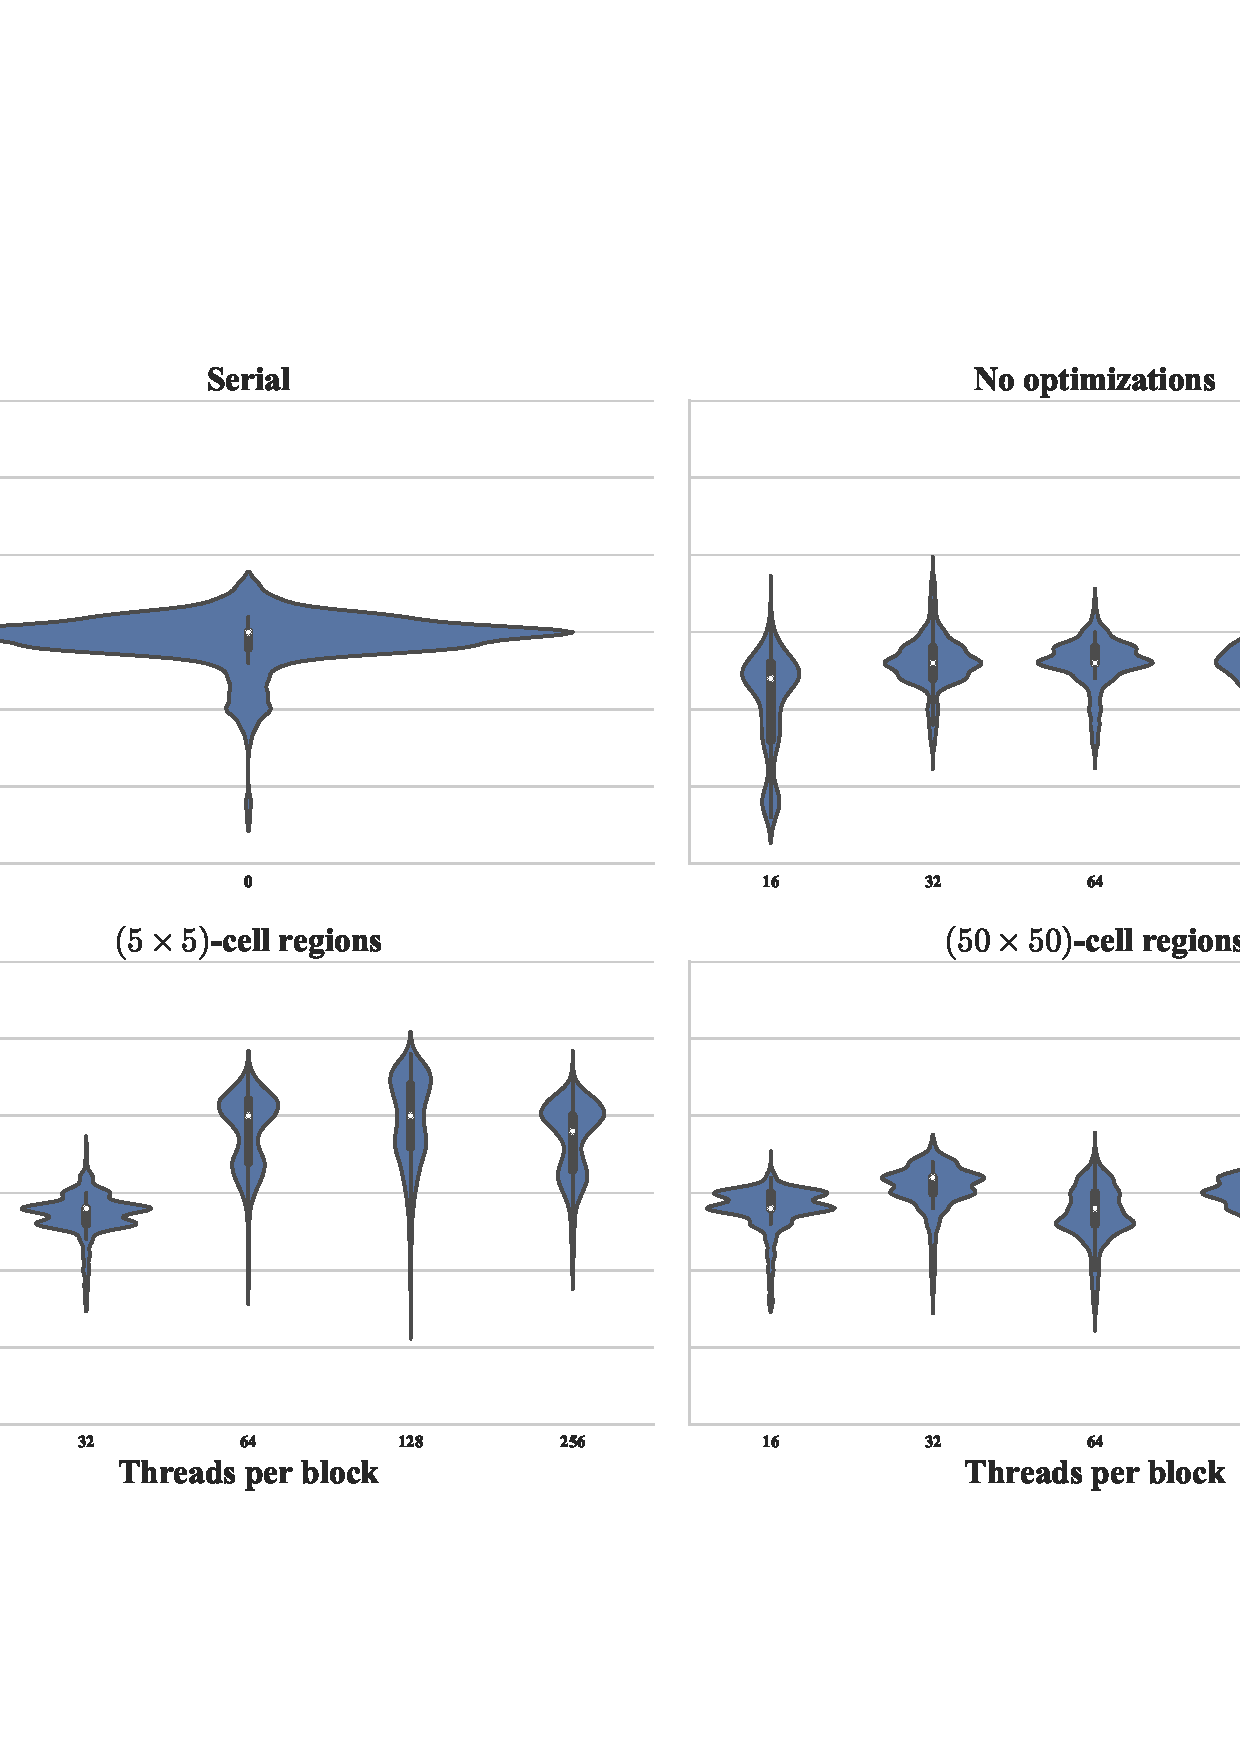
\includegraphics[width=\textwidth]{../images/boxplot.jpg}
        \caption{}
        \label{fig:means}
    \end{figure}

    \begin{table}
        \centering
        \begin{tabular}{llr}
            \toprule
            Region dimension & Threads per block & Mean update time \\ \midrule
            (Serial)  & (Serial)   &  19.514 \\
            0  & 16  &  15.402 \\
            & 32  &  18.040 \\
            & 64  &  17.963 \\
            & 128 &  17.565 \\
            & 256 &  17.644 \\ \midrule
            5  & 16  &  17.589 \\
            & 32  &  18.646 \\
            & 64  &  24.019 \\
            & 128 &  24.675 \\
            & 256 &  23.528 \\ \midrule
            50 & 16  &  18.981 \\
            & 32  &  20.290 \\
            & 64  &  18.633 \\
            & 128 &  19.660 \\
            & 256 & 19.919 \\ \bottomrule
        \end{tabular}
        \caption{[Better caption]}
        \label{tab:means} t
    \end{table}

    \begin{table}
        \centering
        \begin{tabular}{rrrrrr} \toprule
            Region dim 1 &  Region dim 2  &
            Threads/block 1 &  Threads/block 2 &  $t$-statistic & $p$-value \\ \midrule
 5 &   0  & 16 & 128  &   -0.274335&  0.783856 \\
 5 &   0  & 16 & 256  &    0.735564&  0.462082 \\
 0 &   0  & 32 &  64  &   -0.969775&  0.332276 \\
 5 &  50  & 32 &  64  &   -0.165566&  0.868515 \\
 0 &   0  & 128 & 256 &    0.892050 &  0.372473 \\
50 &  -1  & 128 &   0 &   -1.870520 &  0.061558 \\
\bottomrule
\end{tabular}
        \caption{Statistically insignificant 2-sample $t$-test results ($p =
            10^{-2}$).}
        \label{tab:jj}
    \end{table}<++>

\end{document}
